\documentclass[conference]{IEEEtran}
\IEEEoverridecommandlockouts

\usepackage{cite}
\usepackage{amsmath,amssymb,amsfonts}
\usepackage{algorithmic}
\usepackage{graphicx}
\usepackage{textcomp}
\usepackage{xcolor}
\usepackage{tikz}
\usepackage{float}

\def\BibTeX{{\rm B\kern-.05em{\sc i\kern-.025em b}\kern-.08em\kern-.1667em\lower.7ex\hbox{E}\kern-.125emX}}

\begin{document}

\title{Revisiting Rosenblatt’s Perceptron: Robust High-Entropy Classification via Uncertainty Margins}


\author{
    \IEEEauthorblockN{1\textsuperscript{st} Dylan Sutton Chavez}
    \IEEEauthorblockA{\textit{Independent Research} \\
    Mexico City, Mexico \\
    c.sutton.dylan@gmail.com}
}

\maketitle

\begin{abstract}
This paper addresses the challenge of deploying uncertainty-aware models in resource-constrained tiny machine learning environments. While state-of-the-art architectures, such as long short-term memory networks and transformers, provide high representational capacity, their inference overhead and memory requirements are often prohibitive for edge applications. This work develops a computationally efficient alternative: a modified linear perceptron featuring an adaptive selective prediction mechanism. 

By defining a geometric abstention region $[-\epsilon, \epsilon]$ around the decision hyperplane, the model introduces a confidence-aware mechanism and selectively rejects low-confidence samples. Unlike static margin classifiers, the proposed $\epsilon$ parameter is derived from statistical properties estimated during training and calibration \cite{b14}, and it remains fixed during inference, preserving constant-time complexity $\mathcal{O}(d)$.

The framework was evaluated across several high-entropy scenarios, including nonstationary financial time series, sentiment analysis using the Semantic Evaluation dataset, and industrial fault detection based on the National Aeronautics and Space Administration Industrial Machine Surveillance bearing dataset. Experimental results demonstrated that the model achieved an inference memory footprint of $\approx 1$ KB and orders of magnitude lower computational overhead than recurrent neural networks. 

The selective mechanism enables the model to reach precision levels exceeding 90\% at reduced coverage of high-confidence predictions in industrial tasks. These findings suggest that robust feature engineering coupled with selective linear modeling provides an energy-efficient and reliable approach for inference in hardware-limited settings.
\end{abstract}

\begin{IEEEkeywords}
tiny machine learning, simple perceptron, uncertainty quantification, selective prediction, feature engineering, time series forecasting, nonstationary data.
\end{IEEEkeywords}

\section{Introduction}

Modern machine learning models comprise multiple algebraic transformations (i.e., hidden layers) \cite{b15} and exhibit a time complexity greater than $\mathcal{O}(d)$ per prediction, resulting in high computational costs during training, inference, and fine-tuning, particularly in embedded edge applications.

Such models identify patterns in raw data by applying geometric transformations \cite{b2}, processing the input layer by layer to extract increasingly abstract representations.

By contrast, feature learning can be replaced by feature engineering, where mathematical formulations are employed to encode relevant structures directly, rather than relying on hidden layers for representation learning. For example, periodic structures can be efficiently captured using trigonometric functions such as sine and cosine functions to represent circular coordinates.

Following the introduction of the simple perceptron by Rosenblatt in 1958 \cite{b7}, Cover formalized the principle that \textit{``complex pattern classification problems, cast in a high-dimensional space nonlinearly...''} \cite{b2}. This observation suggests that nonlinear projections into higher-dimensional spaces increase the probability of achieving linear separability, enabling simple models to perform effectively in complex pattern recognition tasks.

Accordingly, this work focuses on achieving high-precision inference through selective prediction rather than universal coverage, under strict computational and memory constraints.

\section{Background and Related Work}

\subsection{Background}

Linear models such as the simple perceptron \cite{b7} or linear regression \cite{b4} share the property of computing a linear combination of input features. In classification settings, this linear response is typically mapped to a binary decision.

These models operate under the \textit{``formulation of the general linear combination''} \cite{b4}. In the case of the simple perceptron, the model computes the dot product between the input feature vector ($x_i$) and weight vector ($w_i$), followed by the addition of a bias ($b$) term:

\begin{equation}
z = \sum_{i=1}^{n} w_i x_i + b
\end{equation}

The resulting scalar value is then passed through an activation function. Each model employs a different activation depending on its objectives; for example, the simple perceptron uses a step function to produce a binary output \cite{b7}.

\begin{equation}
\hat{y} = f(z) = \begin{cases} 1 & \text{if } z \geq 0 \\ 0 & \text{if } z < 0 \end{cases}
\end{equation}

However, while individual linear units (weights) are computationally efficient, modern deep neural networks stack multiple layers of these operations, resulting in millions of parameters. This scale presents a challenge for deployment on embedded systems with limited memory.

The mid-20th century experienced a \textit{``machine learning winter''}. Models such as the simple perceptron lacked the geometric capacity to solve problems such as XOR \cite{b6}, leading to the decline of these models, and they were largely used as a foundation for subsequent model generations.

Although the nonlinear limitations of the simple perceptron with respect to the XOR problem led to the prioritization of multilayer architectures \cite{b6}, current energy constraints in edge computing warrant a re-evaluation of linear models when coupled with robust feature engineering.

\subsection{Related Work}

A diverse set of techniques has been developed to quantify model uncertainty \cite{b16}. Bayesian neural networks leverage probabilistic parameters to localize low-confidence regions. However, they typically rely on Monte Carlo sampling during inference, which is computationally prohibitive for micro-controller-based tiny machine learning (TinyML). Similarly, support vector machines (SVMs) optimize a static separation margin with $\mathcal{O}(n^2)$ training complexity, limiting their adaptability to nonstationary data streams.

Other model families, such as ProtoNN and Bonsai \cite{b11}, are tailored for embedded or otherwise resource-limited settings, offering low computational complexity while preserving competitive accuracy. These approaches are often employed in safety-critical domains (e.g., fault diagnosis in engineered systems), where incorrect decisions may lead to serious consequences. To reduce such risks, the proposed uncertainty-aware perceptron follows a similar philosophy, using data dispersion as the basis for quantifying predictive confidence.

Unlike SVMs, which determine a fixed separating margin through a computationally demanding training process with complexity on the order of $\mathcal{O}(n^2)$, the geometric margin $\epsilon$ in the proposed approach is computed from statistical descriptors (e.g., the empirical standard deviation $\sigma$) learned during training and calibration. This design maintains an inference complexity of $\mathcal{O}(d)$, where $d$ is the dimensionality of the input.

Current machine learning research often prioritizes representation learning architectures (e.g., long short-term memory networks or transformers). However, for nonstationary time series, the computational burden of learning temporal dependencies can in many cases be replaced by trigonometric cyclic encoding and stochastic oscillators \cite{b12}. Shifting from learning the structure to explicitly encoding the structure allows linear models to remain competitive in high-entropy settings, especially when selective prediction and reliability-oriented performance metrics are used.

\section{Methods}

This section presents the proposed uncertainty-aware linear perceptron, detailing its decision rule, learning procedure, and feature representation.

\subsection{Uncertainty-Aware Linear Decision Rule}

To quantify uncertainty ($\epsilon$) in the simple perceptron, the geometry of the step function defines the region in which the weighted sum lies for positive (1) and negative (0) predictions.

The modified decision function is defined as

\begin{equation}
h(z) =
\begin{cases}
1   & \text{if } z > \epsilon \\
0   & \text{if } z < -\epsilon \\
0.5 & \text{if } -\epsilon \leq z \leq \epsilon.
\end{cases}
\end{equation}

The introduction of the region $[-\epsilon, \epsilon]$ transforms the usual decision into a geometric margin. Following the principles established by Cortes and Vapnik, maximizing the distance of data points from the separating hyperplane improves generalization \cite{b9}. This approach is consistent with modern selective classification strategies that prioritize precision over coverage \cite{b13}.

Fig. 1 illustrates the modified step function with the uncertainty margin $\epsilon$, highlighting the abstention region around the decision boundary.

\begin{figure}[H]
    \centering
    \caption{Uncertainty-Step-Function}
    \label{fig:Uncertainty-Step-Function}
    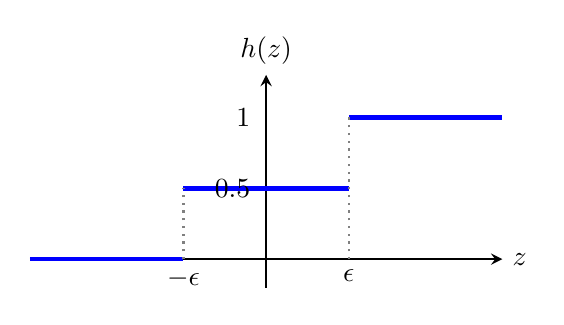
\begin{tikzpicture}[x=1.5cm, y=1.8cm, thick, >=stealth]
        \draw[->] (-2,0) -- (2,0) node[right] {$z$};
        \draw[->] (0,-0.2) -- (0,1.3) node[above] {$h(z)$};
    
        \def\ep{0.7}
    
        \draw[blue, ultra thick] (-2,0) -- (-\ep,0) (-\ep,0.5) -- (\ep,0.5) (\ep,1) -- (2,1);
    
        \draw[gray, dotted] (-\ep,0) node[below, black]{$-\epsilon$} -- (-\ep,0.5);
        \draw[gray, dotted] (\ep,0)  node[below, black]{$\epsilon$}  -- (\ep,1);
    
        \node[left, xshift=-2pt] at (0,0.5) {$0.5$};
        \node[left, xshift=-2pt] at (0,1) {$1$};
    \end{tikzpicture}
\end{figure}

Unlike static margins in SVMs, the proposed $\epsilon$ introduces an uncertainty-aware margin, forcing the perceptron to continue updating its weights when samples fall within the uncertainty region ($h(z) = 0.5$), indicating insufficient geometric distance from the decision boundary.

The uncertainty parameter ($\epsilon$) is a constant defined prior to each prediction, introducing a gray region around the decision boundary. The model outputs a positive prediction (1) when the linear activation ($z$) exceeds the uncertainty threshold ($\epsilon$). 

When $z$ is below the negative region, the prediction is negative (0). If neither condition is satisfied, the prediction falls in the uncertainty region, yielding an indeterminate or outlier-like case (0.5).

To compute the uncertainty margin of the model, the standard deviation ($\sigma$) is proposed, which Karl Pearson defined as \textit{``...a natural measure of the `scatter' of observations.''} \cite{b10}. 

In high-dimensional spaces, the standard deviation ($\sigma$) indicates the level of dispersion and noise in the data; this quantity is computed over the training samples projected onto the model hyperplane, where the uncertainty margin $\sigma$ is estimated during training and calibration and remains fixed during inference.

\begin{equation}
\sigma = \sqrt{\frac{1}{N} \sum_{i=1}^{N} (x_i - \mu)^2}
\end{equation}

The proposed formula to compute model uncertainty begins by defining an external margin to calibrate the model sensitivity ($\Delta$), obtained by scaling the standard deviation ($\sigma$) by the training error rate $E \in [0,1]$. 

This function, based on a Gaussian formulation, adjusts the confidence of the model as a function of the observed error rate ($\text{E} = (\text{Number of Errors in Training} / \text{Total Attempts}) * 100\%$). When the error rate is low, the predictions of the model become more reliable; conversely, higher error rates indicate a reduced confidence.

\begin{equation}
\epsilon = \Delta \cdot \sigma \cdot Z_{(1 - \frac{E}{2})}
\end{equation}

Where $Z_{(1 - \frac{E}{2})}$ represents the critical value of the standard normal distribution corresponding to the desired confidence level, allocating a probability of $\frac{E}{2}$ to each tail of the distribution.

\subsection{Learning Rule}

During each learning epoch, the model updates its parameters using the perceptron learning rule \cite{b7}. The weight adjustment is calculated as the product of the learning rate ($\eta$) and the prediction error, defined as the difference between the true label ($y$) and the predicted output of the perceptron ($\hat{y}$), which is obtained from the activation step function.

The weight update rule (for each weight $w$) is defined as

\begin{equation}
w_i \leftarrow \eta (y - \hat{y}) x_i.
\end{equation}

Similarly, the bias ($b$) is updated as follows:

\begin{equation}
b \leftarrow b + \eta (y - \hat{y}).
\end{equation}

\subsection{Vectorization and Feature Representation}

To construct an algebraic representation for linear modeling, the raw time series data are transformed into a structured input vector using a set of operations.

The objective of this vectorization process is to represent diverse temporal, statistical, and dynamical properties of the signal in a high-dimensional space, thereby increasing the probability of achieving linear separability.

The resulting input vector ($v$) is composed of three characteristic groups: indicators that capture the structure of the time series, cyclic time encoding to preserve the periodicity, and normalized statistical attributes to ensure the appropriate data scaling.

\subsubsection{Nonstationary Indicator Features}

Here, the raw data vector is $x$. A set of indicators is used as statistical metrics to represent the temporal behavior and condition of the data.

The results presented in this work are obtained using a specific set of indicators, which introduce nonlinear transformations of the original raw values, expanding the representational capacity of the linear model.

Each element of vector $x$ is denoted by $x_i$; the maximum and minimum values are given by $x_{\max}$ and $x_{\min}$, and the last element is denoted by $x_n$.

The stochastic oscillator is defined as

\begin{equation}
\%K = \frac{x_n - x_{\min}}{x_{\max} - x_{\min}} \cdot 100.
\end{equation}

Given the vector $x$, the positive and negative gradients are computed as separate sequences. The gain vector $G$ is defined such that $G_i$ contains positive changes and zero otherwise. By contrast, the negative gradient vector $L$ contains the absolute value of negative changes and zero otherwise.

Relative strength (RS) is computed as

\begin{equation}
RS = \frac{\frac{1}{n} \sum_{i=1}^{n}G_i}{\frac{1}{n} \sum_{i=1}^{n}L_i}.
\end{equation}

From which the relative strength index (RSI) is derived:

\begin{equation}
RSI = 100 - \frac{100}{1 + RS}.
\end{equation}

To capture temporal smoothing and exponential decay, the exponential moving average (EMA) is computed as

\begin{equation}
EMA_{\text{initial}} = SMA = \frac{\sum_{i=1}^{n}x_i}{n},
\end{equation}

\begin{equation}
EMA_t = EMA_{t-1} + \alpha(x_n - EMA_{t-1}),
\end{equation}

with smoothing factor

\begin{equation}
\alpha = \frac{2}{n + 1}.
\end{equation}

In the representation of cyclic time encoding, the model encodes the temporal position (e.g., month, week, hour). The model uses these functions to represent the coordinates in the selected timestamp.

\begin{equation}
v = \frac{2\pi \cdot t}{T}
\end{equation}

\begin{equation}
\sin(v), \quad \cos(v)
\end{equation}

The z-score normalization is implemented to scale the external values using a consistent scale (computed across the training dataset partition), where $\sigma$ represents the standard deviation of $x$.

\begin{equation}
z = \frac{x_n - (\frac{1}{n} \sum_{i=1}^{n} x_i)}{\sigma}
\end{equation}

Although a significant amount of work is done through feature engineering, the proposed model remains capable of filtering noise, finding a high-dimensional hyperplane, and identifying a noise pattern within the data, all achieved through the model’s fine-tuning capabilities.

\section{Experimental Setup}

The following section describes the datasets, evaluation protocol, and hardware configuration used to assess the proposed method.

\subsection{Datasets}

\subsubsection{Nonstationary Financial Time-Series Dataset}

During training, various high-noise-level and nonstationary datasets were used for model testing. To validate the model in environments where large amounts of data are easily available, several historical corporate datasets were selected.

These datasets were chosen because corporate time-series environments allow the model to be subjected to sustained noise stress over long periods (up to ten years).

\subsubsection{Sentiment Analysis Dataset and Data Preprocessing}

To demonstrate that this model is not limited to long nonstationary data, it was also challenged using a dataset for sentiment analysis, classified as positive (1) or negative (0). The dataset selected for this task was SemEval; https://semeval.github.io/, which provides sentiment labels for social media text, demonstrating the applicability of the proposed model when applied to natural language processing tasks.

For data preparation, n-grams were used and a corresponding scale was created to normalize the token values between 0 and 1. Finally, for data analysis, techniques similar to those used in convolutional neural networks were applied, where the model operates in a manner similar to a sliding window over the sequence, performing inference depending on the size of the respective input vector.

\subsubsection{Industrial Validation: NASA IMS Bearing Dataset}

To further validate the model in a critical embedded sensing scenario, the NASA IMS Bearing Dataset was used. This task involves  binary classification of bearing condition (healthy (1) vs. faulty (0)) based on vibration accelerometer data; https://data.nasa.gov/dataset/ims-bearings.

Unlike the stochastic nature of markets, mechanical degradation follows physical laws; however, early fault detection remains challenging owing to signal noise during transitional degradation states. For this task, a low-dimensional input vector is engineered, consisting of root mean square (RMS), harmonic oscillators, sin, cos, kurtosis, crest factor, and skewness, computed over sliding windows.

\subsection{Data Management and Evaluation Protocol}

\subsubsection{Dataset Splitting}

To ensure proper data collection and avoid data leakage, the entire dataset was divided into separate subsets for training ($73\%$) and post-training evaluation ($27\%$).

A sliding window algorithm (using a window length of 14 samples) was implemented to iterate over the current and past observation window. The model was constrained to prevent access to future data.

\subsubsection{Sliding-Window Evaluation}

With the split dataset, the model was trained using the standard perceptron learning procedure, following the Rosenblatt approach \cite{b7}. After completion of the full training phase, the uncertainty mechanism was applied during post-training evaluation, and the model was run across the entire dataset using the same sliding window approach.

\subsection{Hardware Configuration}

The hardware used during training consisted of a single 64-bit CPU core and approximately 1 MB of RAM. During the inference phase, the model used only approximately 1 kB of memory because it did not need to load the dataset into memory.

Similarly, the model was tested on a t2.micro instance within the Amazon Web Services (AWS) architecture. Running on this hardware, the same resource usage characteristics were observed.

\section{Results}

\subsection{Nonstationary Time Series Results}

The section presents the results obtained from experiments conducted across multiple high-noise environments, together with the computational resources employed and the corresponding approximate execution times, including data post-processing, training, and inference. 

The statistical properties of the nonstationary datasets used in this study are summarized in Table~\ref{tab:Timestamp-Window-Sequential-Set}. 

Table~\ref{tab:Training-Time-Sequential-Set} reports the total training time and number of training vectors for each dataset. Baseline training accuracy without selective prediction is reported in Table~\ref{tab:Total-Accuracy-Sequential-Set}. 

Finally, Table~\ref{tab:Uncertainty-Accuracy-Medium} presents the coverage--accuracy trade-off obtained after introducing the uncertainty mechanism.

\begin{table}[H]
    \centering
    \caption{Dataset Signal Profiles \& Characteristics}
    \label{tab:Timestamp-Window-Sequential-Set}
    \begin{tabular}{c c c}
        \hline
        Dataset ID & Volatility Profile ($\sigma$) & Duration (years)\\
        \hline
        Type I & $0.58$ & $2.75$\\
        Type II & $0.31$ & $9.5$\\
        Type III & $0.23$ & $7.3$\\
        Type IV & $0.26$ & $2.9$\\
        \hline
        \multicolumn{3}{p{0.9\linewidth}}{\centering
        Sampled at 15 min time steps. $\sigma$ represents the annualized standard deviation of the datasets, characterizing signal volatility. Type I: Tesla (TSLA), Type II: Alphabet (GOOGL), Type III: Eli Lilly and Company, Type IV: Apple Inc. (AAPL).
        }
    \end{tabular}
\end{table}

\begin{table}[H]
    \centering
    \caption{Training Time}
    \label{tab:Training-Time-Sequential-Set}
    \begin{tabular}{c c c}
        \hline
        Dataset Type & Time (seconds) & Training Vectors\\
        \hline
        Type I & $3.34$ sec & $40000$\\
        Type II & $9.44$ sec & $110000$\\
        Type III & $6.14$ sec & $80000$\\
        Type IV & $3.74$ sec & $37000$\\
        \hline
        \multicolumn{3}{p{0.9\linewidth}}{\centering
        The obtained results include data processing and preprocessing time incurred during training.
        }
    \end{tabular}
\end{table}

\begin{table}[H]
    \centering
    \caption{Total Training Accuracy (in all the dataset, without uncertainty)}
    \label{tab:Total-Accuracy-Sequential-Set}
    \begin{tabular}{c c}
        \hline
        Dataset Type & Total Accuracy ($\%$)\\
        \hline
        Type I & $56.1$\\
        Type II & $55.31$\\
        Type III & $56.34$\\
        Type IV & $56.84$\\
        \hline
        \multicolumn{2}{p{0.9\linewidth}}{\centering
        The dataset was split into $73\%$ for training and $27\%$ for testing.
        }
    \end{tabular}
\end{table}

These tables present the coverage–accuracy trade-off obtained on the evaluation partition after incorporating the uncertainty mechanism under different sensitivity settings.

\begin{table}[H]
    \centering
    \caption{Uncertainty Accuracy in a Small Coverage}
    \label{tab:Uncertainty-Accuracy-Small}
    \begin{tabular}{c c c}
        \hline
        Dataset Type & Coverage ($\%$) & Accuracy ($\%$)\\
        \hline
        Type I & $17$ & $97$\\
        Type II & $23$ & $93$\\
        Type III & $21$ & $89$\\
        Type IV & $23$ & $93$\\
        \hline
        \multicolumn{3}{p{0.9\linewidth}}{\centering
        Overview of the performance achieved on the low-coverage data, illustrating the impact of the uncertainty function across different sensitivity thresholds.
        }
    \end{tabular}
\end{table}

\begin{table}[H]
    \centering
    \caption{Uncertainty Accuracy in a Medium Coverage}
    \label{tab:Uncertainty-Accuracy-Medium}
    \begin{tabular}{c c c}
        \hline
        Dataset Type & Coverage ($\%$) & Accuracy ($\%$)\\
        \hline
        Type I & $47$ & $68$\\
        Type II & $43$ & $67$\\
        Type III & $52$ & $68$\\
        Type IV & $42$ & $69$\\
        \hline
        \multicolumn{3}{p{0.9\linewidth}}{\centering
        Performance summary for the medium-coverage scenario, showing how accuracy adjusts when the uncertainty function is applied.
        }
    \end{tabular}
\end{table}

\subsection{Sentiment Analysis Results}

The performance in the SemEval sentiment classification task is summarized in Table~\ref{tab:NLP-SemEval}.

\begin{table}[H]
    \centering
    \caption{Natural Language Processing Results}
    \label{tab:NLP-SemEval}
    \begin{tabular}{c c c}
        \hline
        Metric & Value & Notes\\
        \hline
        Total Coverage & $83.4\%$ Acc. & N/A\\
        Selected Coverage & $97.7\%$ Acc. & $79.3\%$ Coverage\\
        Model Dimensions & 1080 & N/A\\
        Training Time & $9$ sec & N/A\\
        \hline
        \multicolumn{3}{p{0.9\linewidth}}{\centering
        This table reports total and selected coverage, model dimensionality (corresponding to the number of n-grams or bag-of-words features), and training time.
        }
    \end{tabular}
\end{table}

\subsection{Industrial Data Results}

The proposed model demonstrated high efficiency in this domain, effectively filtering transitional noise to provide a reliable early warning capability. Table~\ref{tab:NASA-Results} reports accuracy and coverage results on the NASA IMS Bearing Dataset.

\begin{table}[H]
    \centering
    \caption{Performance on NASA Bearing Dataset}
    \label{tab:NASA-Results}
    \begin{tabular}{c c c}
        \hline
        Metric & Value & Notes\\
        \hline
        Total Coverage & $89.4\%$ Acc. & N/A\\
        Selected Coverage & $94.7\%$ Acc. & $88.5\%$ Coverage\\
        Model Dimensions & 14 & N/A\\
        Training Time & $6.4$ sec & N/A\\
        \hline
        \multicolumn{3}{p{0.9\linewidth}}{\centering
        By rejecting uncertain samples during transient degradation phases, the model achieved high accuracy in confirmed states, supporting robust low-power early warning operation.
        }
    \end{tabular}
\end{table}

\section{Analysis and Comparison}

This section analyzes the computational implications of the obtained results and situates the proposed approach relative to existing TinyML models.

\subsection{Computational Complexity Analysis}

The primary distinction of the proposed model lies in its reduced time complexity and minimal memory footprint. Before the formal analysis, this section describes the underlying mathematical foundations and the analytical formulations for each component of the model. A comparison of time complexity across models is provided in Table~\ref{tab:Mathematical-Analysis}.

\begin{table}[H]
    \centering
    \caption{Time Complexity and Memory Space}
    \label{tab:Mathematical-Analysis}
    \begin{tabular}{c c c}
        \hline
        Stage & Time Complexity & Memory Space\\
        \hline
        Training & $\mathcal{O}(e \cdot n \cdot d)$ & $\mathcal{O}(d)$\\
        Inference & $\mathcal{O}(d)$ & $\mathcal{O}(d)$\\
        Input Vector & $\mathcal{O}(d \cdot l)$ & $\mathcal{O}(d)$\\
        Uncertainty Function & $\mathcal{O}(1)$ & $\mathcal{O}(1)$\\
        \hline
        \multicolumn{3}{p{0.9\linewidth}}{\centering
        e = epochs, n = samples, d = features, l = length
        }
    \end{tabular}
\end{table}

\subsection{Comparison}

Following the methodology described in this paper, a comparative analysis is presented with various machine learning architectures. This evaluation focuses on time complexity ($\mathcal{O}$), memory complexity (memory footprint), and operational performance in high-entropy environments.

For this comparison, Bonsai \cite{b11}, FastGRNN \cite{b12}, and ProtoNN \cite{b11} were selected based on their reported performance in TinyML benchmarks. Theoretical training and inference time complexity for each model is summarized in Table~\ref{tab:Time-Complexity-Comparation}. Estimated memory usage and inference latency across models are reported in Table~\ref{tab:Estimated-Hardware-Usage-Comparation}.

Finally, a comparison of sentiment classification performance on the SemEval dataset is shown in Table~\ref{tab:NLP-SemEval-Comparation}.

\begin{table}[H]
    \centering
    \caption{Time Complexity}
    \label{tab:Time-Complexity-Comparation}
    \begin{tabular}{c c c}
        \hline
        Model & Training & Inference\\
        \hline
        Proposed & $\mathcal{O}(e \cdot n \cdot d)$ & $\mathcal{O}(d)$\\
        Bonsai & $\mathcal{O}(e \cdot n \cdot d  \cdot depth)$ & $\mathcal{O}(d \cdot depth)$\\
        FastGRNN & $\mathcal{O}(e \cdot n \cdot d \cdot l)$ & $\mathcal{O}(d \cdot l)$\\
        ProtoNN & $\mathcal{O}(e \cdot n \cdot d \cdot k)$ & $\mathcal{O}(d \cdot k)$\\
        Linear SVM & $\mathcal{O}(n^2 \cdot d)$ & $\mathcal{O}(d)$\\
        Standard LSTM & $\mathcal{O}(e \cdot n \cdot l \cdot d^2)$ & $\mathcal{O}(l \cdot d^2)$\\
        \hline
    \end{tabular}
\end{table}

\begin{table}[H]
    \centering
    \caption{Estimated Hardware Usage}
    \label{tab:Estimated-Hardware-Usage-Comparation}
    \begin{tabular}{c c c}
        \hline
        Model & Space in Memory (RAM) & Latency\\
        \hline
        Proposed & $1$ KB & $9$ ms\\
        Bonsai & $4.5$ KB & $13$ ms\\
        FastGRNN & $47$ KB & $12$ ms\\
        ProtoNN & $16$ KB & $13$ ms\\
        Linear SVM & $2$ KB & $10$ ms\\
        Standard LSTM & $>500$ KB & $13$ sec\\
        \hline
        \multicolumn{3}{p{0.9\linewidth}}{\centering
        Benchmarks were conducted on a constrained virtualized environment (a single-core 64-bit CPU, a 1 MB RAM limit) to simulate resource scarcity in embedded systems. The reported latency includes the time required for feature preprocessing.
        }
    \end{tabular}
\end{table}

\begin{table}[H]
    \centering
        \caption{Natural Language Tasks (SemEval Dataset)}
    \label{tab:NLP-SemEval-Comparation}
    \begin{tabular}{c c c}
        \hline
        Model & Total Accuracy & Coverage/Accuracy\\
        \hline
        Proposed & $83.4\%$ & $79.3\%$ Cov. and $97.7\%$ Acc.\\
        Bonsai & $69.8\%$ & N/A\\
        FastGRNN & $70.8\%$ & N/A\\
        ProtoNN & $68.4\%$ & N/A\\
        Linear SVM & $67.2\%$ & N/A\\
        Standard LSTM & $87.1\%$ & N/A\\
        \hline
    \end{tabular}
\end{table}

\section{Implications and Future Work}

Current research efforts focus on extending this uncertainty mechanism from a passive filtering mechanism to an active learning trigger, a framework referred to as \textit{Epsilon Recurrent Feedback for Linear Models}.

Although the present work uses $\epsilon$ to abstain from prediction, future iterations aim to leverage the uncertainty region as a routing mechanism to bridge the gap between linear and deep model representations. The proposed framework envisions a hierarchical architecture in which uncertainty-driven decision routing enables adaptive escalation to more expressive models \cite{b17}.

\begin{itemize}

    \item Selective Escalation: Input vectors falling within the uncertainty margin ($\epsilon$) are not discarded; instead, they are escalated to a high-capacity model (e.g., a transformer or large language model) acting as a teacher model.
    
    \item Closed-Loop Distillation: The high-confidence labels generated by the teacher model for these difficult samples are fed back into the linear model. This creates a continuous distillation cycle, allowing the simple perceptron to progressively approximate the decision boundaries of more expressive architectures while maintaining fixed-time $\mathcal{O}(1)$ inference costs for the majority of traffic.
    
    \item Contextual Adaptation: Future work will also explore the integration of context-aware weighting mechanisms using exponential moving averages to handle temporal dependencies without the overhead of recurrent neural networks.
    
\end{itemize}

Preliminary experiments with this feedback mechanism on datasets derived from OWASP benchmarks suggest the potential to compress the knowledge of high-capacity models into linear weights, thereby addressing the linear–deep trade-off for resource-constrained environments.

\section{Conclusion}

This work presented an uncertainty-aware linear perceptron model designed for highly resource-constrained edge environments. The model demonstrated a training complexity of $\mathcal{O}(e \cdot n \cdot d)$ and constant-time inference cost of $\mathcal{O}(d)$, using approximately 1 kB of memory. Furthermore, feature preprocessing exhibited linear complexity $\mathcal{O}(n)$, allowing operations within 100-byte memory buffers. The results empirically illustrate Cover's theorem, effectively suppressing noise in high-entropy environments. 

Crucially, the model prioritizes high precision over universal coverage($>90\%$) through selective coverage. This approach offers orders-of-magnitude reductions in computational costs compared to recurrent neural networks, indicating that robust feature engineering coupled with selective linear modeling is a viable path for reliable TinyML deployment.

\section{Acknowledgment}

Appreciations expressed to the NASA Prognostics Center of Excellence for providing the IMS Bearing Dataset and to the SemEval organizers for making their sentiment analysis datasets available for research. Editorial support, including English editing and proofreading, was provided by Editage.

\section{Resources}

To support reproducibility and further research on resource-constrained machine learning, the complete source code for the Uncertainty-Aware Linear Perceptron is available on GitHub: https://github.com/dylan-sutton-chavez/uncertainty-simple-perceptron/blob/main/src/model/perceptron.py. The repository includes the implementation of the core model, uncertainty step function and the manual feature engineering pipeline for nonstationary time series.

\begin{thebibliography}{00}
\bibitem{b1} K. Cho et al., ``Learning phrase representations using RNN encoder-decoder for statistical machine translation,'' in Proc. Conf. Empir. Methods Nat. Lang. Process., Doha, Qatar, Oct. 2014, pp. 1724–-1734.
\bibitem{b2} T. M. Cover, ``Geometrical and statistical properties of systems of linear inequalities with applications in pattern recognition,'' IEEE Trans. Electron. Comput., vol. EC-14, no. 3, pp. 326--334, June 1965.
\bibitem{b3} S. Hochreiter and J. Schmidhuber, ``Long Short-Term Memory,'' Neural Comput., vol. 9, no. 8, pp. 1735-–1780.
\bibitem{b4} A. M. Legendre, ``Nouvelles méthodes pour la détermination des orbites des comètes,'' 1805.
\bibitem{b5} F. T. Liu, K. M. Ting, and Z. H. Zhou, ``Isolation forest,'' in Proc. IEEE Int. Conf. Data Min., Pisa, Italy, 2008, pp. 413--422.
\bibitem{b6} M. Minsky and S. Papert, ``Perceptrons: An Introduction to Computational Geometry,'' The MIT Press, 1969.
\bibitem{b7} F. Rosenblatt, ``The perceptron: A probabilistic model for information storage and organization in the brain,'' Psychol. Rev., vol. 65, no. 6, pp. 386-–408, 1958.
\bibitem{b8} S. Tuli, G. Casale, and N. R. Jennings, ``TranAD: Deep transformer networks for anomaly detection in multivariate time series,'' in Proc. VLDB Endow., Feb. 2022, pp. 1201--1214.
\bibitem{b9} C. Cortes and V. Vapnik, ``Support-vector networks,'' Mach. Learn., vol. 20, pp. 273--297, 1995.
\bibitem{b10} K. Pearson, ``Contributions to the Mathematical Theory of Evolution,'' Philos. Trans. A Math Phys. Eng. Sci., vol. 185, pp. 71-–110, 1894.
\bibitem{b11} A. Kumar, S. Goyal, and M. Varma, ``Resource-efficient Machine Learning in 2 KB RAM for the Internet of Things,'' in Proc 34th Int. Conf. Mach. Learn., 2017, pp. 1935--1944.
\bibitem{b12} A. Kusupati et al., ``FastGRNN: A Fast, Accurate, Stable, and Tiny RNN for Edge Computing,'' in Proc. 32nd Annu. Conf. Neural Inf. Process. Syst., Montreal, Canada, Dec. 2018.
\bibitem{b13} Y. Geifman and R. El-Yaniv, ``Selective classification for deep neural networks,'' in Proc. 31st Annu. Conf. Neural Inf. Process. Syst., Long Beach, CA, USA, Dec. 2017.
\bibitem{b14} Alexander C., ``Loss: A Notion of Error in Machine Learning,'' J. Hist. Knowl., vol. 6, no. 1, 2025.
\bibitem{b15} Ronny H., Michael S., ``A brief introduction to deep learning,'' in Deep Learning for Synthetic Aperture Radar Remote Sensing, M. Schmitt and R. Hänsch, Eds. Oxford, UK: Elsevier, 2025, pp. 25–52.
\bibitem{b16} S. Wang et al., ``A Survey on Uncertainty Quantification Methods for Deep Learning,'' ACM Comput. Surv., vol. 57, no. 12, 2025.
\bibitem{b17} J. Kim, M. S. Kim, J. H. Park, and J. Kim, ``Uncertainty-Aware Deep Reinforcement Learning Approach for Computational Molecular Design,'' Ind. Eng. Chem. Res., vol. 64, no. 5, 2025.
\end{thebibliography}

\end{document}
